% ERA-Großpraktikums: Benutzeranleitung -- Features

\section{Features}

\subsection*{Überblick}
\todo[inline]{Am besten mit Bild und nummerierten Pfeilen}

% Ich schlage eine Teilung der einzelnen Features nach Projektverwaltung(Laden, Speichern, Snapshots), Erstellen von Programmen (Editor, Hilfetexte), Ausführung von Programmen(Ausfühmodi, Breakpoints), Interaktion mit laufenden Programmen (Input/Output-Components) und sonstiges vor

\subsection{Projekt}

\subsubsection{Projekt erstellen}
\todo[inline]{V.a. Projekt erstellen: Auswahl Architektur, Bitlänge, Modlue, Parser, etc.}
\begin{figure}[ht]
	\centering
  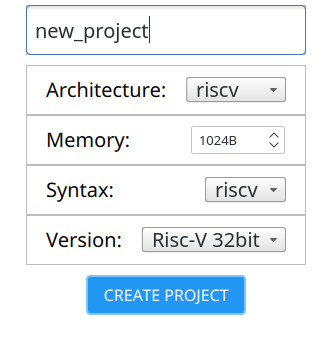
\includegraphics[width=\textwidth]{Images/create_new_project}
	\caption{Erstellen eines neuen Projekts}
	\label{Project_Creation}
\end{figure}


\subsubsection{Speichern/Laden}
\todo[inline]{Speichern/Laden von Projekt und Code}

\subsubsection{Snapshots}
\todo[inline]{Speichern/Laden + Was ist das?; Welche Eigenschaften muss mein erstelltes Projekt haben, damit ich SnapshotXY laden kann (passende Architektur/passende Module)}


\subsection{Erstellen von Programmen}

\subsubsection{Editor}
\todo[inline]{Alles zum Editor (zoomen, Makros aufklappen, Fehlermeldungen anzeigen, Tooltips etc)}

\begin{figure}[ht]
	\centering
  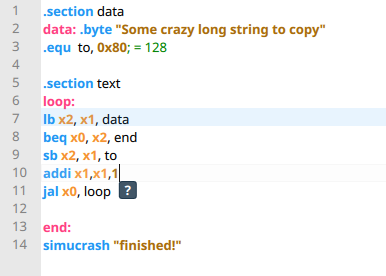
\includegraphics[scale=1]{Images/Editor}
	\caption{der Programmeditor}
	\label{Editor}
\end{figure}


\subsubsection{Hilfetextkomponente}
\todo[inline]{Was wird angezeigt, zu welchem Befehl (Zeile!), wann (nach dem Parsen)}


\subsection{Ausführung von Programmen}

\subsubsection{Ausführungsmodi}
\todo[inline]{komplett, schritt-für-schritt, zum nächsten breakpoint; hier am besten mmit bildern der einzelnen Knöpfe}

\subsubsection{Registerkomponente}
Die Registerkomponente zeigt die Prozessorregister an und ermöglicht es, deren Werte manuell zu verändern. Jedes Register besteht aus einem Registertitel, mit dem es in der Regel auch im Assemblercode referenziert werden kann, sowie dem zugehörigem Registerinhalt.

Der Registerinhalt kann je nach Art des Registers unterschiedlich formatiert werden. Allzweckregistern stehen die Formate \textit{Binär}, \textit{Hexadezimal}, \textit{Dezimal (vorzeichenbehaftet)} und \textit{Dezimal (nicht vorzeichenbehfatet)} zur Verfügung. Ein-Bit Flag-Register können außerdem als Checkbox angezeigt werden.
Die Einstellung der Formate erfolgt über den Button, der sich rechts vom Registertextfeld befindet. Beachten Sie, dass für ein Register unter Umständen nicht alle Format-Optionen zur Verfügung stehen --- so kann der Programmzähler etwa nicht im Dezimal-Format angezeigt werden.

Um den Wert eines Registers manuell zu ändern, wird der Text im Textfeld bearbeitet und die Eingabe mit Enter bestätigt. Auf die Einhaltung der Formatierung wie etwa der Leerzeichen bei Byte-Grenzen muss nicht geachtet werden. Nach Bestätigung der Eingabe wird der Registerwert automatisch der aktuellen Einstellung entsprechend formatiert. Ist etwa ein eingegebener Wert zu lang um im Register gegebener Größe gespeichert werden zu können, werden die höherwertigen überschüssigen Zeichen entfernt. Zudem wird der Registerinhalt durch höherwertige Nullen auf seine Maximalgröße aufgefüllt. Ungültige Zeichen werden automatisch entfernt. Die Registerwerte erhalten im Binär-Format den Präfix ``0b'', im Hexadezimal-Format den Präfix ``0x''.

Über das Einstellungsmenü der Registerkomponente (erreichbar über die Kopfzeile der Komponente) können alle Register auf einmal formatiert werden. Steht das gewählt Format für ein Register nicht zur Vergügung (bspw. Dezimal für den Programmzähler), so behält dieses seine ursprüngliche Formatierung bei.

Einige Register können je nach Architektur festverdrahtet sein und können deshalb weder über eine Assemblerinstruktion noch manuell geändert werden. Die Textfelder dieser Register sind deaktiviert.

Führt man eine einzelne Zeile aus, die den Wert eines Registers ändert, so wird dieses farblich hinterlegt, um die Änderung schnell nachvollziehen zu können.


\subsubsection{Speicherkomponente}
Der Haupspeicher spielt bei allen Programmen eine sehr wichtige Rolle.
Dort sind sowohl der assemblierte Programmcode, der Callstack, als auch Daten zum Arbeiten hinterlegt.
Der Speicher ist dabei in Zellen unterteilt, die in der Regel 1 Byte groß sind.
Auch der Simulator hat natürlich einen solchen RAM, der sich flexibel an die Bedürfnisse des Nutzers anpassen lässt.

\begin{figure}[ht]
	\centering
  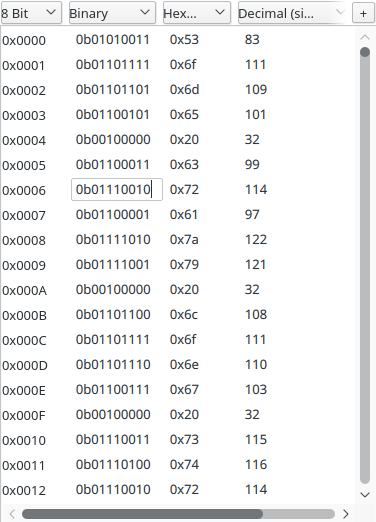
\includegraphics[scale=1]{Images/Memory}
	\caption{der Programmspeicher - RAM}
	\label{Memory}
\end{figure}

Um den Inhalt des Speichers auf einen Blick erfassen zu können, stehen verschieden Einstellungen in der Kopfzeile zur Verfügung:\\
In der ersten Spalte stehen immer die Adressen der Speicherzellen. 
Bei großen Datenmengen ist es manchmal wünschenswert mehr als nur 1 Byte pro Zeile angezeigt zu bekommen.
Deshalb kann im Menu oberhalb dieser Spalte die angezeigte Größe der Speicherzellen eingestellt werden.
Standardmäßig stehen hier $8\, Bit$, $16\, Bit$, $32\, Bit$ und $64\, Bit$ zur Auswahl. 
Dabei wird aber die die architekturbedingte Größe der Speicherzellen nicht beeinflusst; es werden stattdessen mehrere Speicherzellen pro Zeile dargestellt.
Deshalb ändert sich die angezeigte Adressierung entsprechend.\\
Des Weiteren stehen mehrere Anzeigeformate für den Inhalt zur Verfügung, welche jeweils oberhalb einer angezeigten Spalte ausgewählt werden können.
Dabei stehen standardmäßig ``Binär'', ``Hexadezimal'', ``Dezimal'' und ``Dezimal (vorzeichenbehaftet/signed)'' zur Verfügung. 
Letzteres kann den Speicherinhalt auch als negative Zahl interpretieren bzw. auch negative Eingaben entgegen nehmen. \\
Außerdem können die Inhalte der Speicherzellen nebeneinander gleichzeitig in verschiedenen Formaten repräsentiert werden.
Dazu einfach auf das ``\texttt{+}'' in der rechten oberen Ecke klicken. Daraufhin erscheint eine neue Spalte im Speicher, 
bei der auch wieder das Format ausgewählt werden kann. Um eine Spalte wieder zu entfernen, muss in dem Auswahlfeld für das Format der letzte
Eintrag ``\texttt{remove...}'' ausgewählt werden.

\begin{warningblock}
Bei einer ungültigen Eingabe wird die Zahl bestmöglich interpretiert und anstelle des
eingegebenen Wertes an die Speicherstelle geschrieben. Dazu zählt auch die Eingabe zu großer Zahlen.
Die Ersetzung erfolgt sofort.
\end{warningblock}


\subsection{Interaktion mit laufenden Programmen}
\todo[inline]{Hier sollte (für alle Komponenten ja gleich) die Einstellungsmöglichkeiten (Zahnrad-knopf) und welches Symbol welche Komponente bedeutet}

\subsubsection{Eingabe -- Pfeiltasten}
\todo[inline]{v.a. welche Werte werden für welchen Pfeil geschrieben}
\begin{figure}[ht]
	\centering
  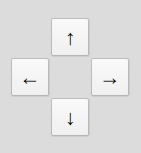
\includegraphics[width=0.2\textwidth]{Images/Joystick}
	\caption{Eingabe mit Pfeiltasten}
	\label{Joystick}
\end{figure}


\subsubsection{Eingabe -- Mausklick}
\todo[inline]{welche werte werden geschrieben, Reihenfolge?}

\subsubsection{Eingabe -- Text}
\todo[inline]{wann wird geschriebener Text in den Speicher geschrieben?, Wie lang kann mein Text sein?}

\subsubsection{Ausgabe -- Lichtbandanzeige}
\todo[inline]{besondere Einstellungen! Farbwahl! Manuelles setzen der Strips möglich!}
\begin{figure}[ht]
	\centering
  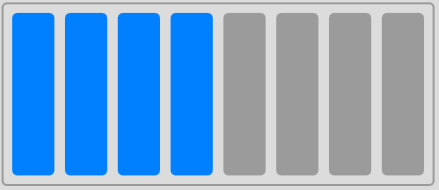
\includegraphics[width=0.8\textwidth]{Images/Lightstrip}
	\caption{Leuchtbandanzeige}
	\label{Lightstrip}
\end{figure}

\begin{figure}[ht]
	\centering
  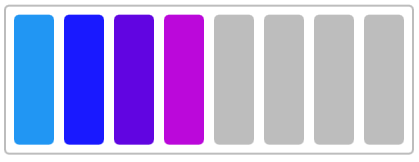
\includegraphics[width=0.8\textwidth]{Images/Lightstrip_colors}
	\caption{Leuchtbandanzeige mit verschiedenen Farben}
	\label{Lightstrip_Colors}
\end{figure}


\subsubsection{Ausgabe -- 7-Segmentanzeige}
Die sogenannte 7-Segment Anzeige ist eine einfache alphanumerische Ausgabe, 
wie sie häufig bei kleinen digitalen Geräten zum Einsatz kommt.
Anzeige besteht, wie der Name schon sagt, aus 7 Strichen, die unabhängig voneinander zum Leuchten gebracht werden können.

\begin{figure}[ht]
	\centering
  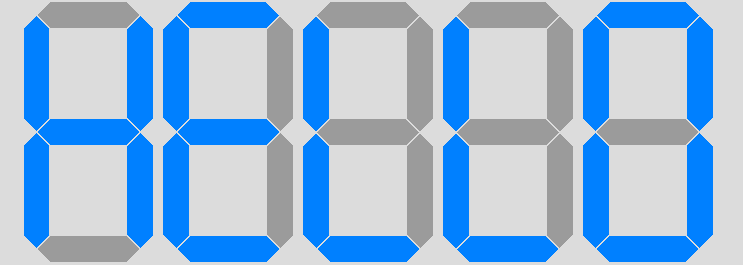
\includegraphics[width=0.8\textwidth]{Images/7-Segment_Hello}
	\caption{Die 7-Segment Anzeige im Simulator}
	\label{7-Segment}
\end{figure}

Jedes dieser Segmente wird durch ein einzelnes Bit angesteuert. Dabei bedeutet $1$, dass das Segment leuchten soll und $0$ entsprechend, dass es nicht leuchten soll.
Pro Zeichen wird somit 8 Byte zum Ansteuern benötigt, wobei das höchstwertige Bit in der Regel ignoriert wird.

Wenn man die Maus im Simulator über ein Zeichen bewegt, erscheint dort die Reihenfolge, in der die Bits den einzelnen Segmenten zugeordnet sind.

\begin{figure}[ht]
	\centering
  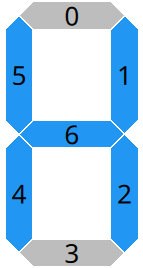
\includegraphics[width=0.2\textwidth]{Images/7-Segment_Hover}
	\caption{Die Reihenfolge der Bits}
	\label{7-Segment_Hover}
\end{figure}

Es können auch gleichzeitig mehrere Zeichen angesteuert werden. Die einzelnen Bytes für jedes Zeichen stehen dann im Speicher an aufeinanderfolgenden Adressen.
Dabei muss aber darauf geachtet werden, dass die Reihenfolge genau umgedreht ist. Das Zeichen am rechten Rand steht somit an der ersten Adresse im Speicher, 
danach folgt das vorletzte usw.

\begin{warningblock}
Reihenfolge der Zeichen: Die Ansteuerung der Zeichen ist genau geschieht (wie im Zahlensystem) von rechts nach links. 
\end{warningblock}

Ein kleines Beispiel verdeutlicht dies wohl am besten.

\begin{exampleblock}{HELLO}
	Für das oben gezeigte \texttt{HELLO} wäre also folgende Ansteuerung nötig:\\
	\begin{tabular}{llll}
	0x3f & 0b00111111 & & \texttt{O}\\
	0x38 & 0b00111000 & & \texttt{L}\\
	0x38 & 0b00111000 & & \texttt{L}\\
	0x79 & 0b01111001 & & \texttt{E}\\
	0x76 & 0b01110110 & & \texttt{H}\\
	\end{tabular}
\end{exampleblock}

Falls man sich den Umweg über die Ansteuerung über Speicheradressen sparen möchte, 
kann man die einzelnen Leuchtsegmente auch durch einen Klick mit der linken Maustaste aktivieren bzw. deaktivieren. 

Für die Anzeige gibt es zwei Einstellungen, die man über das Zahnrad rechts unten aufrufen kann:\\
\begin{itemize}
\item \texttt{Memory Source (Address):} definiert den Speicherbereich, der für die 7-Segment Ausgabe herangezogen wird. Default ist 0.
\item \texttt{Number of Digits:} die Anzahl der angezeigten 7-Segment Zeichen. Für jedes der Zeichen wird ein Byte im Speicher benötigt. 
					Die Bytes für jedes Zeichen sind im Speicher an aufeinanderfolgenden Adressen ab der gewählten  \texttt{Memory Source Address} angeordnet.
\end{itemize}



\subsubsection{Ausgabe -- Konsole}
\todo[inline]{pipe-like, array-based; }


\subsection{Sonstige Features}
